\documentclass[../main.tex]{subfiles}
\graphicspath{{\subfix{../img/}}}
\begin{document}

\newpage
\section{Projektplanung}

\subsection{Risikomatrix} \label{risikomatrix}

Alle bekannten Risiken von dem Projekt sind in folgender Tabelle aufgelistet.
Dabei hat jedes Risiko folgende Attribute:
\begin{itemize}
    \item \textbf{Titel + Beschreibung}: Beschreibung des Risikos
    \item \textbf{Verantwortlich} Welche Gruppe dafür Verantwortlich ist (INF=Informatik, MT=Mechaniker, ET=Elektroniker).
    \item \textbf{Kategorie}: In welcher Kategorie sich das Risiko befindet.
    \item \textbf{Ursachen}: Was passieren muss, damit das Risiko eintreffen kann.
    \item \textbf{Bewertung des Risikos}: Eintrittswahrscheinlichkeit, Auswirkung und Risiko Bewertung ohne Massnahmen
    \item \textbf{Massnahmen zur Risikominimierung}: Massnahmen um die Eintrittswahrscheinlichkeit oder Auswirkung zu minimieren.
    \item \textbf{Korrekturmassnahmen}: Was gemacht werden soll, wenn das Risiko trotzdem Eintrifft
    \item \textbf{Erfolgsfaktoren}: Beschreibt das Verhalten bei erfolgreicher Risikomitigation
    \item \textbf{Erneute Bewertung des Risikos}: Eintrittswahrscheinlichkeit, Auswirkung und Risiko Bewertung mit den definierten Massnahmen
\end{itemize}

Aus Darstellungsgründen wurden die Attribute der Risiko in zwei Tabellen aufgeteilt.

\begin{landscape}
\newpage
\scriptsize

\textbf{Legende:}
\hspace{1cm}
\textbf{VW:} Verantwortlich
\hspace{1cm}
\textbf{EW:} Eintrittswahrscheinlichkeit (1-5)
\hspace{1cm}
\textbf{AW:} Auswirkung (1-5)
\hspace{1cm}
\textbf{BW:} Bewertung (EW * AW)

\begin{longtable}{|c|p{4cm}|p{6cm}|c|c|p{4cm}|c|c|c|}
\hline
\textbf{ID}  & \textbf{Titel} & \textbf{Beschreibung} & \textbf{VW} & \textbf{Kategorie} & \textbf{Ursachen} & \textbf{EW} & \textbf{AW} & \textbf{BW} \\ \hline
R1  & Grip-Verlust normale Räder & Das Fahrzeug schleift über den Boden & MT & Mechanisch & Fahrzeug verliert Grip & 3 & 3 & 9 \\ \hline
R2  & Liniensensor falsche Daten & Der Liniensensor erkennt die Fugen als Führungslinie & ET+INF & Elektrisch & Fahrzeug folgt der Fuge & 4 & 4 & 16 \\ \hline
R3  & Motorenposition ungenau & Für Rückstellen des Hindernis ungenau Positionswerte & ET & Elektrisch & Hindernis nicht innerhalb 2 cm & 3 & 3 & 9 \\ \hline
R4  & Distanzmessung fehlerhafte Daten & Für die Erkennung der Distanz, des Hindernis, könnten falsche Messwerte eine ungewollte Aktion ausführen & ET & Elektrisch & Fahrzeug führt Hindernisbewältigung aus ohne ein Hindernis & 2 & 2 & 4 \\ \hline
R5  & Datenverlust & Verlust von Projektdaten/Forschungsergebnissen & INF & Projekt & Server offline & 2 & 5 & 10 \\ \hline
R6  & Lieferschwierigkeiten & Teile, die bestellt werden haben Lieferverzögerung, was zur Verzögerung im jeweiligen Test-/Integrationsprozess führt & Market & & Längere Lieferzeiten/Keine Lieferzeiten angegeben & 3 & 4 & 12 \\ \hline
R7  & Software-Absturz & Software crasht während Einsatz & INF & Software & Prozess wird unerwartet beendet & 2 & 5 & 10 \\ \hline
R8  & Verlust Sensorkommunikation & Die Kommunikation zwischen Sensorik und Software ist gestört & ET+INF & Software & Fehlerhafte Daten oder fehlende Daten & 2 & 5 & 10 \\ \hline
R9  & Software zu anspruchsvoll für Computer & Die Leistung des Computers reicht nicht für die Echtzeitverarbeitung der Algorithmen & INF & Software & Software-Lags, langsame Reaktionszeit & 3 & 4 & 12 \\ \hline
R10 & Pylone wird überfahren & Eine Pylone wird nicht erkannt und überfahren & ET+INF & Elektrisch & Pylone wird nicht erkannt & 3 & 5 & 15 \\ \hline
R11 & Unscharfe Bilder während Fahrt erschweren Objekterkennung & Die Kamera bewegt sich während der Fahrt zu stark und liefert unscharfe Bilder & MT+INF & Software & Objekterkennung findet keine Objekte oder an falschen Orten & 4 & 4 & 16 \\ \hline
R12 & Fokus der Kamera umfasst nicht ganzen benötigten Bereich & Bilder enthalten unscharfe Teile, da die Focus Range nicht den ganzen benötigten Bereich umfasst. (Von Fahrzeug zu nächstem Punkt (Max 2m)) & ET+INF & Elektrisch & Teile des Bilds unscharf und Objekte werden nicht korrekt erkannt & 3 & 3 & 9 \\ \hline
R13 & Grip Verlust Omni und Mecanum & & & Mechanisch & Fahrzeug verliert Grip bei den Fugen & 4 & 4 & 16 \\ \hline
R14 & Anzahl GPIO & Die Steuerungselektronik hat eine begrenzte Anzahl IN/OUT Pins & ET & Elektrisch & Sensorinformationen können nicht gelesen werden & 3 & 5 & 15 \\ \hline
R15 & Verschiebung bei Drehung & Mit dem Fahrantrieb kann keine genaue Drehung an Ort und Stelle realisiert werden, um das Fahrzeug mit dem aufgenommenen Hindernis zu wenden. & MT & Mechanisch & Fahrzeug schiebt zur Seite bei Drehung & 3 & 5 & 15 \\ \hline
\end{longtable}

\newpage

\textbf{Legende:}
\hspace{1cm}
\textbf{EW:} Eintrittswahrscheinlichkeit mit Massnahmen (1-5)
\hspace{1cm}
\textbf{AW:} Auswirkung mit Massnahmen  (1-5)
\hspace{1cm}
\textbf{BW:} Bewertung mit Massnahmen (EW * AW)

\begin{longtable}{|c|p{7cm}|p{5cm}|p{5cm}|c|c|c|}
\hline
\textbf{ID} & \textbf{Massnahmen Risikominderung} & \textbf{Korrekturmassnahmen} & \textbf{Erfolgsfaktoren} & \textbf{EW} & \textbf{AW} & \textbf{BW} \\ \hline
R1  & Auf Mensaboden testen & Andere Räder/Geschwindigkeit anpassen & Fahrzeug hat Grip & 2 & 2 & 4 \\ \hline
R2  & Kalibrierung des Sensors, Abgleich mit Kamera. Befahren einer Linie nur, wenn Punkt oder Hindernis am Ende erkannt & Not-Aus verwenden & Fahrzeug folgt Führungslinie & 2 & 5 & 10 \\ \hline
R3  & Langsame Fahrt bei Positionierung & Hallsensor, Drehgeber, Schrittmotor, Beschleunigungssensor & Hindernis innerhalb der 2 cm Toleranz & 2 & 2 & 4 \\ \hline
R4  & Distanzwert muss längere Zeit konstant bleiben & Zweiter Sensor zum Vergleich verbauen & Fahrzeug führt Hindernisbewältigung nur bei einem Hindernis aus & 1 & 2 & 2 \\ \hline
R5  & Regelmässige Backups erstellen & Daten aus Backups wiederherstellen & Daten sind zugänglich und schnell wiederherstellbar & 2 & 2 & 4 \\ \hline
R6  & Frühzeitig Bestellen, alternative Teile/Quellen suchen & bei alternativen Quellen bestellen, Alternative Teile nutzen & Teile können zeitnah verwendet verbaut werden & 3 & 3 & 9 \\ \hline
R7  & Gutes Testen des Codes und Failsafe einbauen, der bei Absturz ausgeführt wird. Aktuellen Zustand zwischenspeichern & Not-Aus verwenden & Fahrzeug kann nach Absturz von alleine wieder starten und fortfahren, ohne, dass das Fahrzeug die Linien verlässt & 1 & 5 & 5 \\ \hline
R8  & Sicheres verbauen und Testen der Sensoren. Nominalwerte prüfen und Fehlerzustände definieren, um diese erkennen zu können. In solchen Fällen Neueinstellung/Kalibrierung durchführen & Wege in Software haben, um auch mit fehlender Sensorik die Aufgabe zu erfüllen. & Fahrzeug kann trotz fehlerhafter oder fehlender Sensordaten Aufgabe erfüllen & 2 & 3 & 6 \\ \hline
R9  & Software von Beginn auf für Plattform optimiert bauen. Keine Bewegung des Fahrzeugs, wenn Fahrsteuerung überlastet. & Akzeptieren und langsamer fortsetzen & Fahrzeug kann trotz langsamer Laufzeit die Aufgabe lösen & 3 & 3 & 9 \\ \hline
R10 & Frühes Training und Testing für Pylonenerkennung mit Simulation oder real world data, Backup-Sensor, der bei Nichterkennen von nahem Hindernis Alarm schlägt & Not-Aus verwenden & Das Fahrzeug erkennt Pylonen und fährt sie nicht um & 1 & 5 & 5 \\ \hline
R11 & Bildaufnahme nur bei stehendem Fahrzeug. Training mit verschwommenen Bilddaten. Dafür frühe Datenaufnahme nötig & Fahrzeug für längere Zeit stehen lassen, bis scharfe Bilder da sind & Das Fahrzeug erkennt Objekte und kann mit scharfen Bildern arbeiten & 2 & 4 & 8 \\ \hline
R12 & Im Vorfeld Fokus-Range prüfen und frühzeitig testen. Training mit verschwommenen Bilddaten & Software auf Fälle anpassen, bei denen Fokus-Bereich nicht reicht. & Fahrzeug kann Objekte richtig erkennen & 2 & 2 & 4 \\ \hline
R13 & Testen der Räder & Mit Sensoren Position ausgleichen, dafür eine genaue Position des Fahrzeugs benötigt & Fahrzeug ist an der gewünschten Position & 3 & 3 & 9 \\ \hline
R14 & & & & & & \\ \hline
R15 & Testen & Zusatzfunktion: abdocken und drehen des Fahrzeuges. & Fahrzeug dreht an fixer Position & & & \\ \hline
\end{longtable}

\normalsize
\end{landscape}

TODO: Bild von Risikomatrix

Diese Risiken werden so früh im Projekt wie möglich versucht zu minimieren.
Dies kann beispielsweise anhand von einem Prototypen, Backup Lösungen oder vertiefter Recherche gemacht werden.
\subsubsection{Recherche zu Risiko R16: Blendung der Kamera durch Reflexionen}
Eine Möglichkeit, Reflexionen zu reduzieren, kann im Fotografiebereich mit Polarisationsfiltern gearbeitet werden, die nur Licht mit einer gewissen Polarisierung durchlassen. Mit Hilfe eines bereits vorhandenen Polarisationsfilters wurden Tests gemacht, inwiefern die Reflexionen tatsächlich mit solchen Filtern reduziert werden können.
\begin{table}[h!]
    \centering
    \begin{tabular}{|c|c|c|c|}
        \hline
        \parbox[c][2cm][c]{3cm}{\centering Ohne Polarisationsfilter} & 
        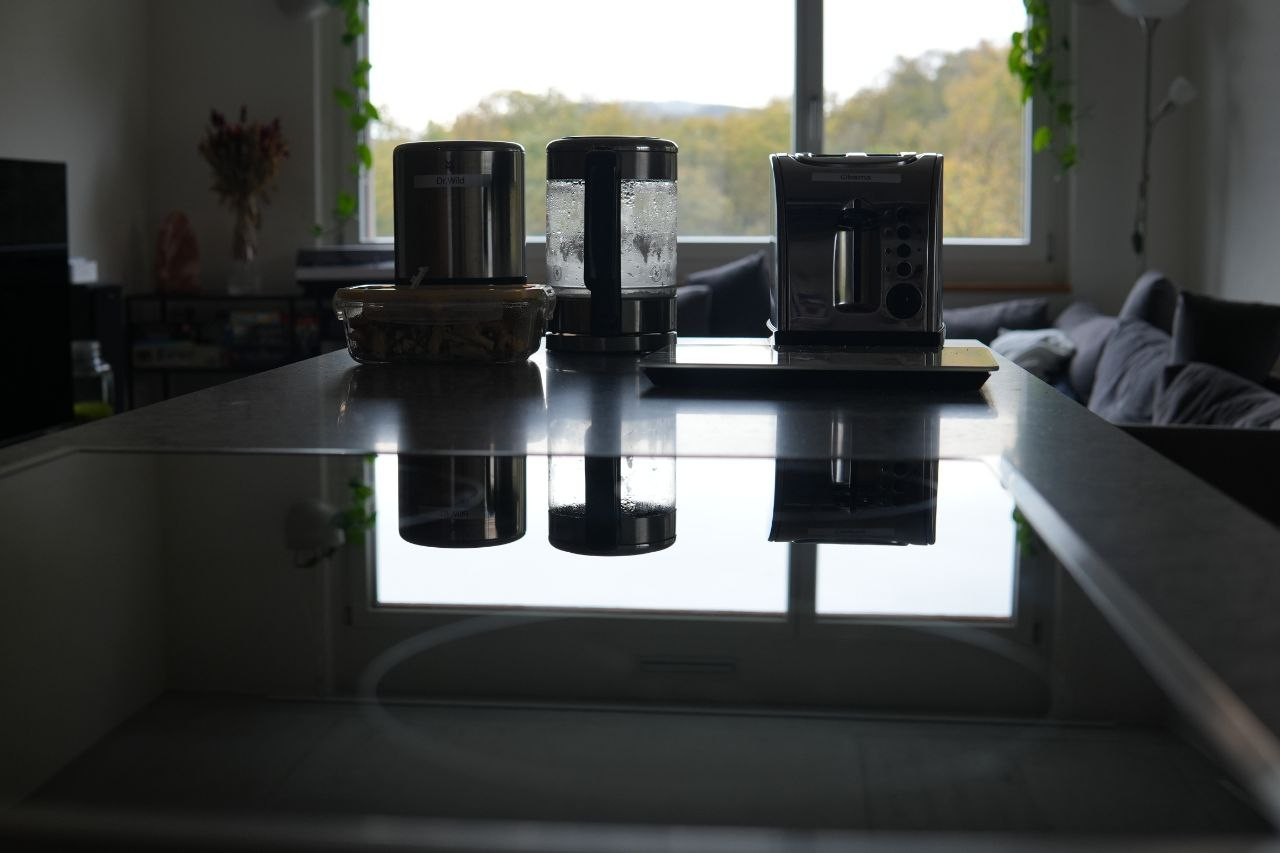
\includegraphics[width=4cm]{img/polarisierungsfilter/pol1_n.jpg} & 
        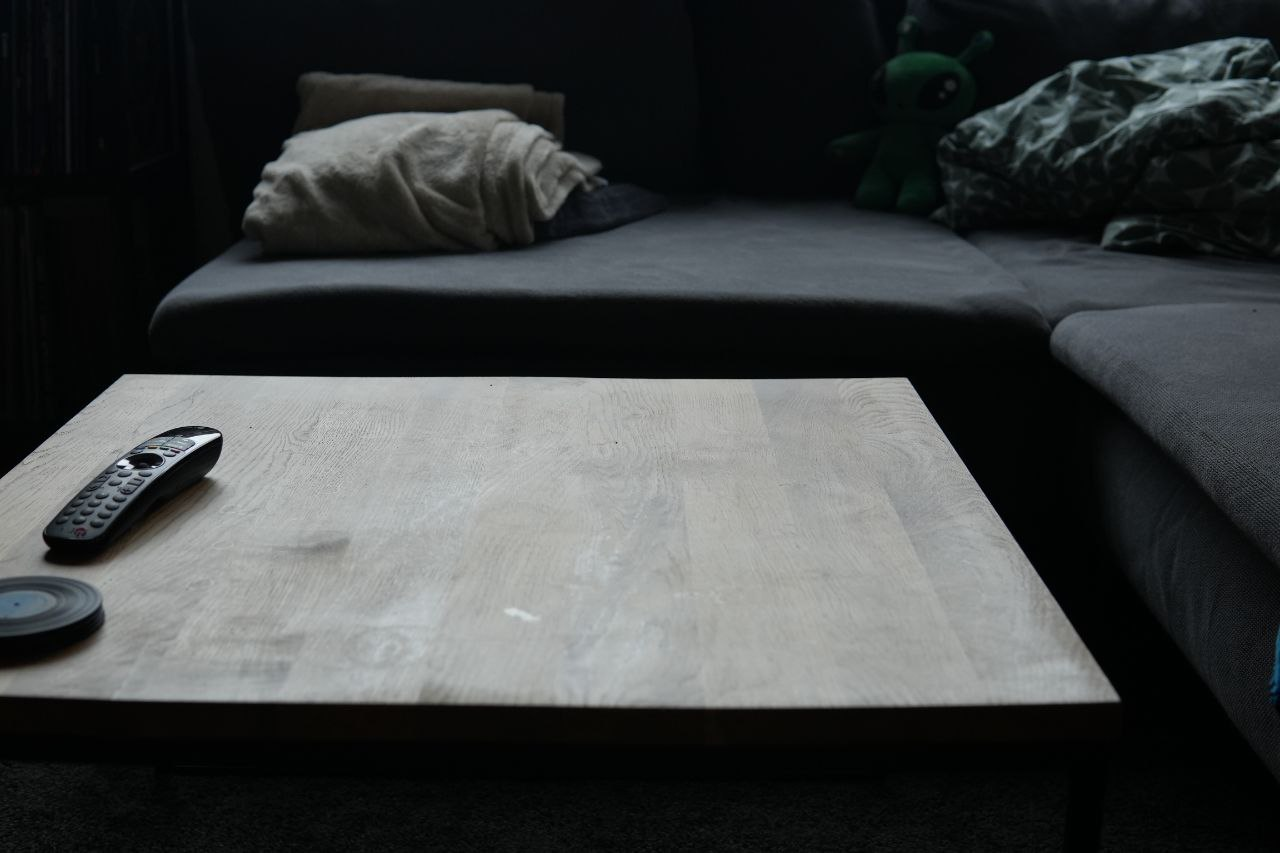
\includegraphics[width=4cm]{img/polarisierungsfilter/pol2_n.jpg} & 
        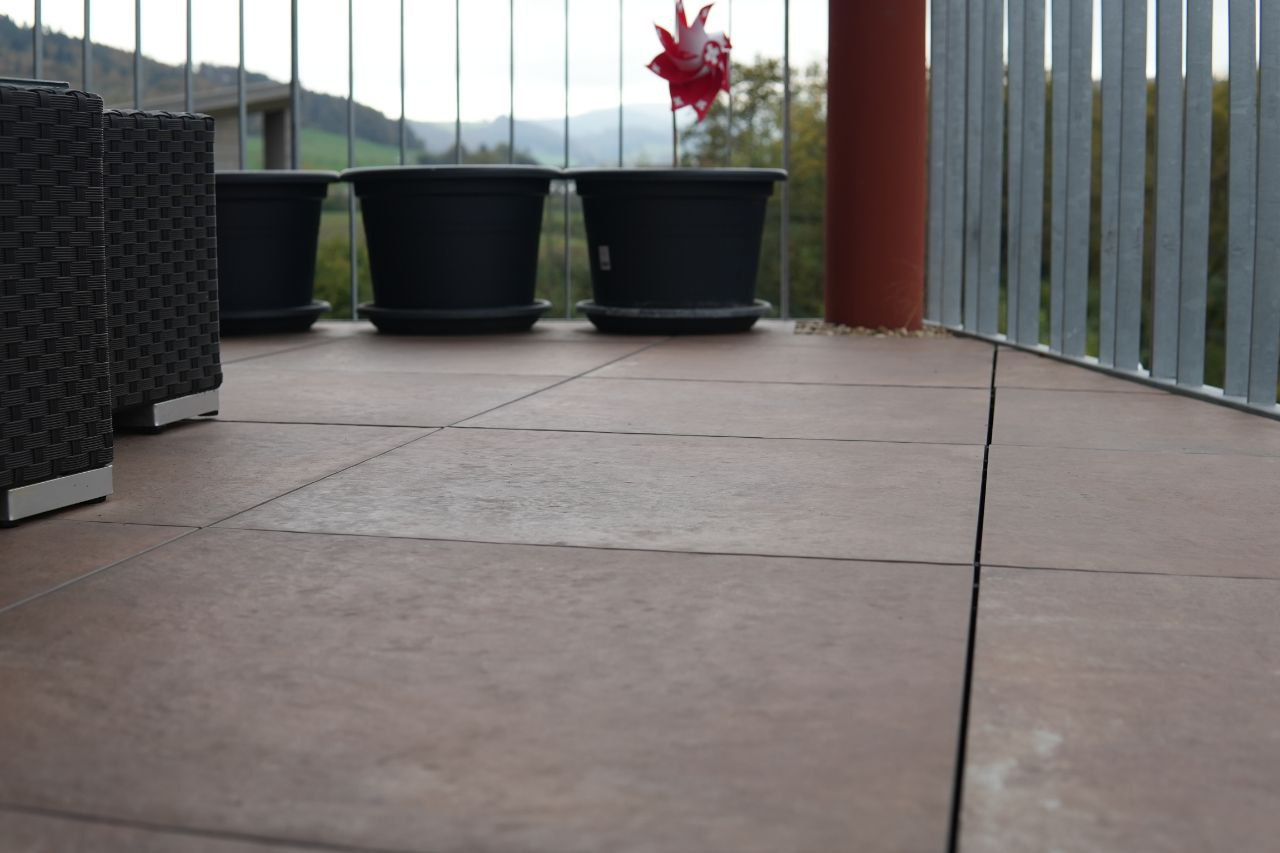
\includegraphics[width=4cm]{img/polarisierungsfilter/pol3_n.jpg} \\
        \hline
        \parbox[c][2cm][c]{3cm}{\centering Mit Polarisationsfilter} & 
        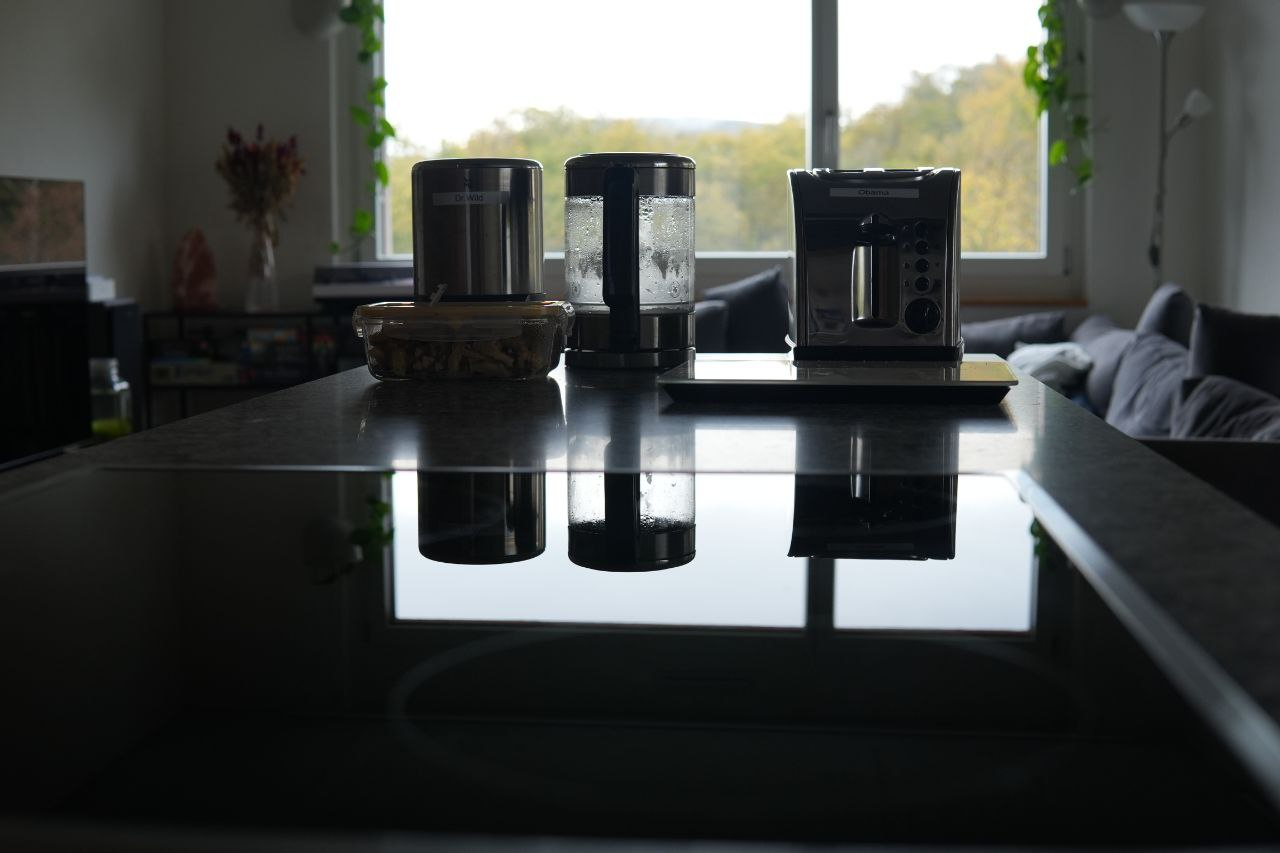
\includegraphics[width=4cm]{img/polarisierungsfilter/pol1_j.jpg} & 
        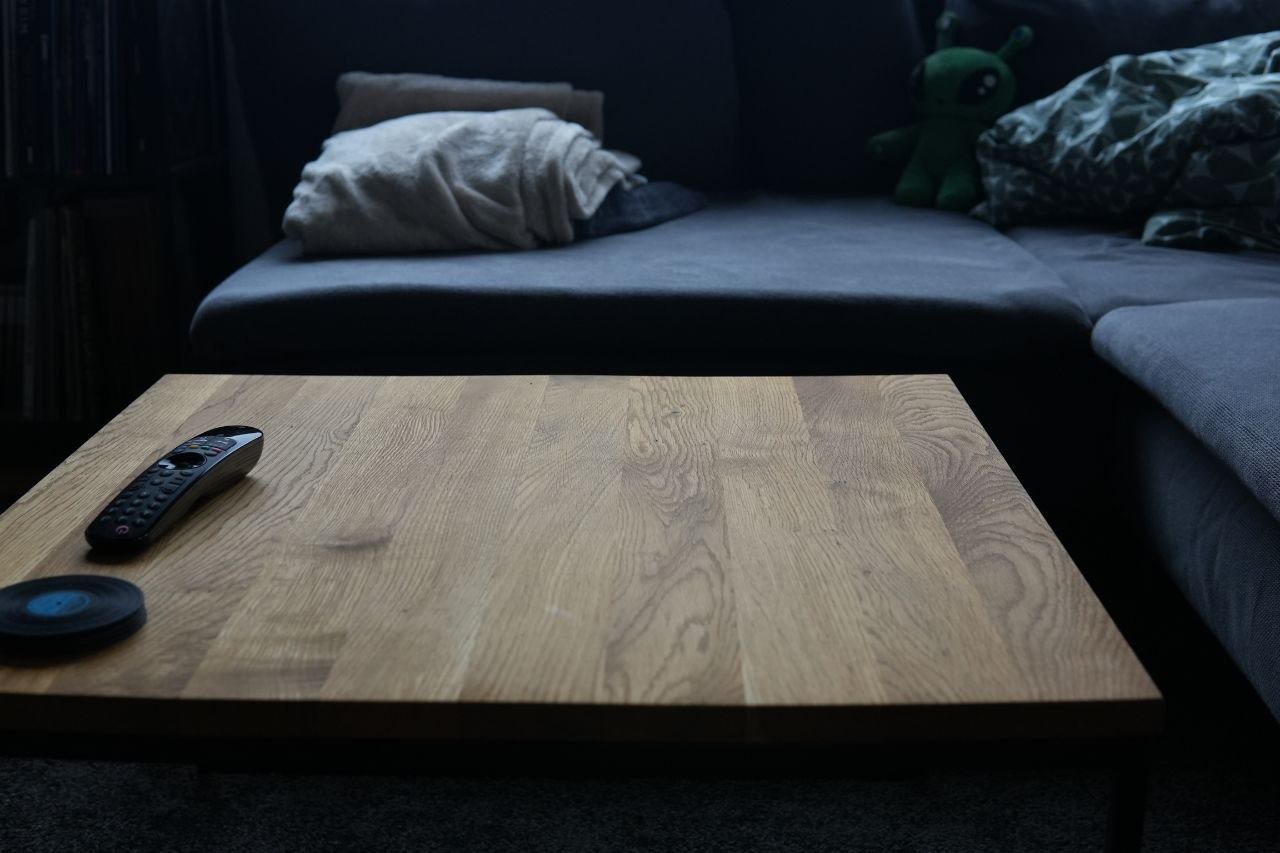
\includegraphics[width=4cm]{img/polarisierungsfilter/pol2_j.jpg} & 
        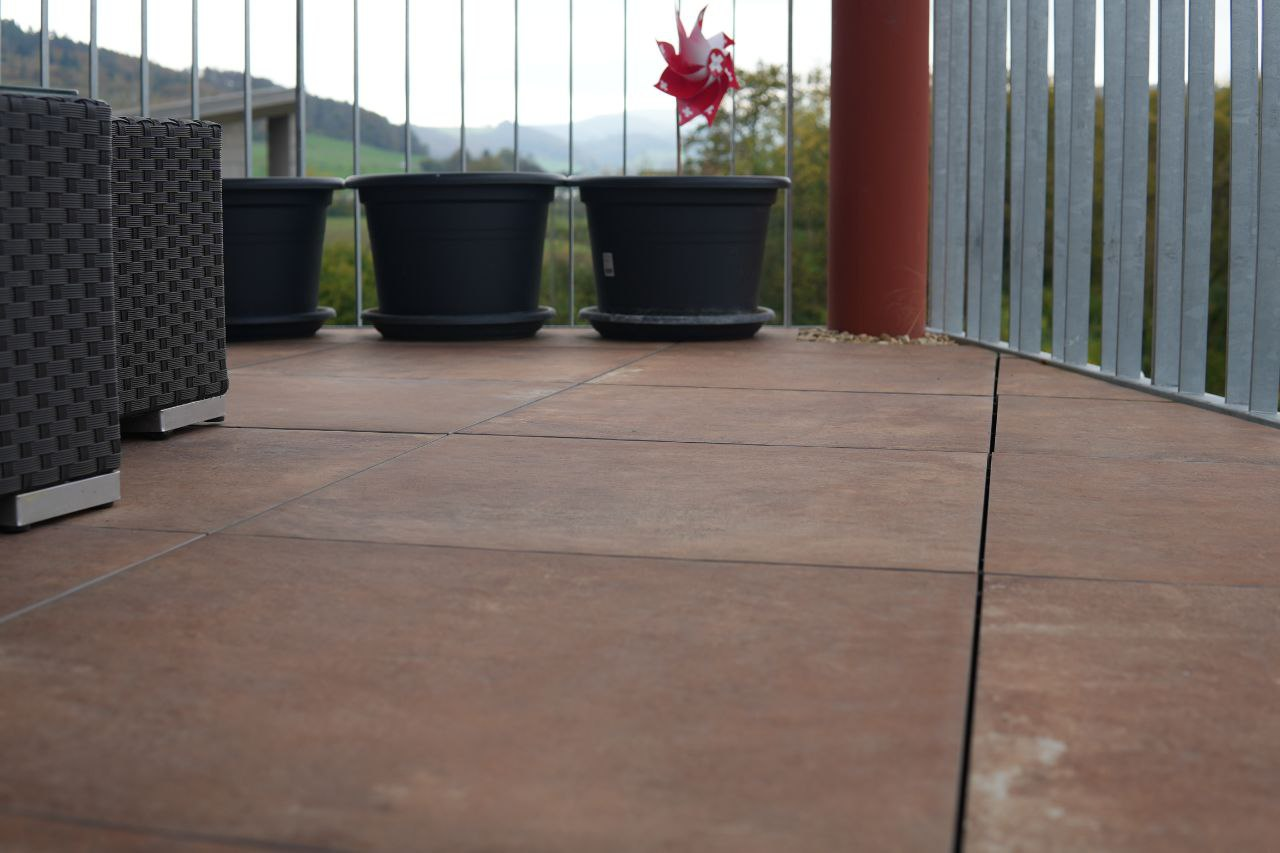
\includegraphics[width=4cm]{img/polarisierungsfilter/pol3_j.jpg} \\
        \hline
    \end{tabular}
    \caption{Vergleich Polarisationsfilter}
\end{table}
Die Resultate sind nicht eindeutig und müssen auf dem Mensaboden verifiziert werden. Wenn ein Effekt zu sehen ist, ist eine klare Reduktion der Reflexionen erkennbar


\addtocounter{subsection}{1}
\addcontentsline{toc}{subsection}{ 4.1   Projektplan}
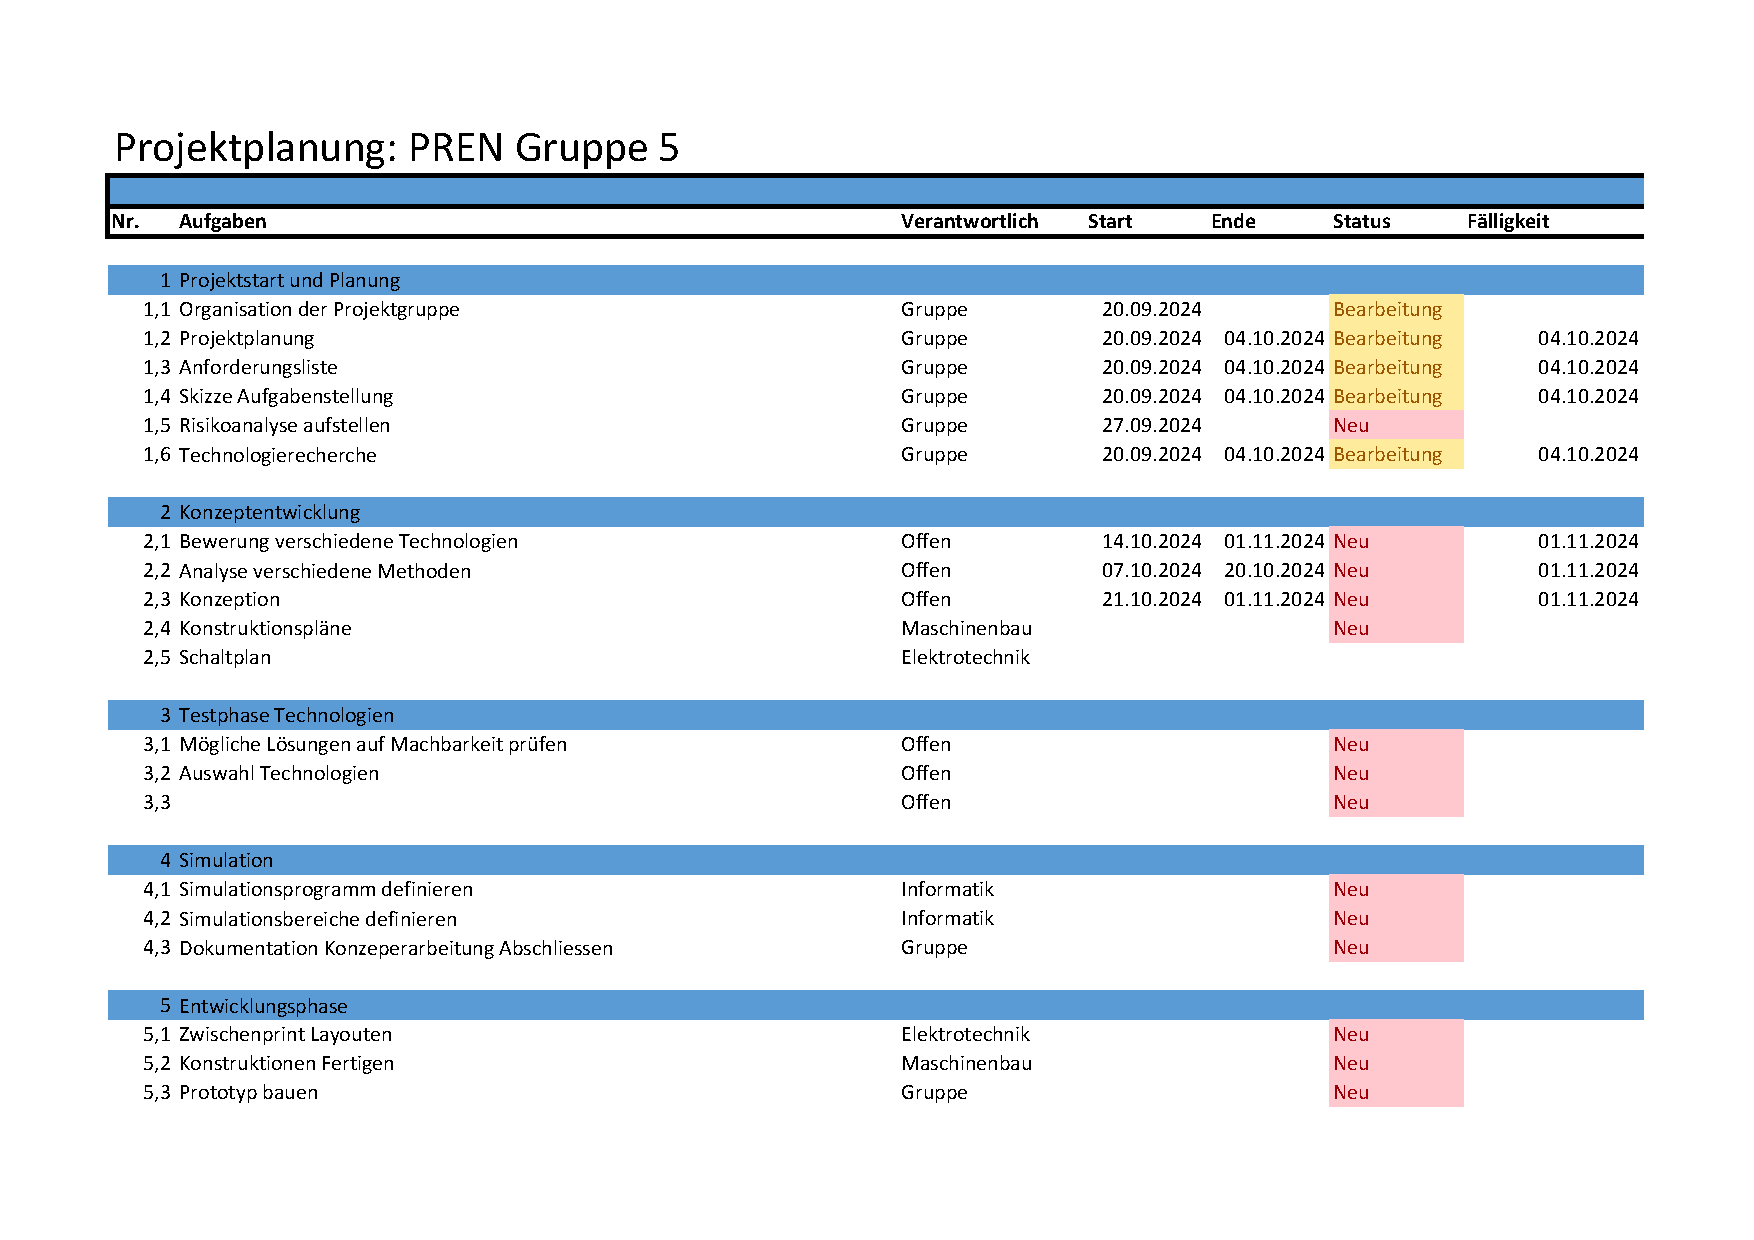
\includepdf[
  landscape=true,
  pages={1-},
  scale=0.9,
  pagecommand={\pagestyle{fancy}}
]{assets/Projektplan.pdf}

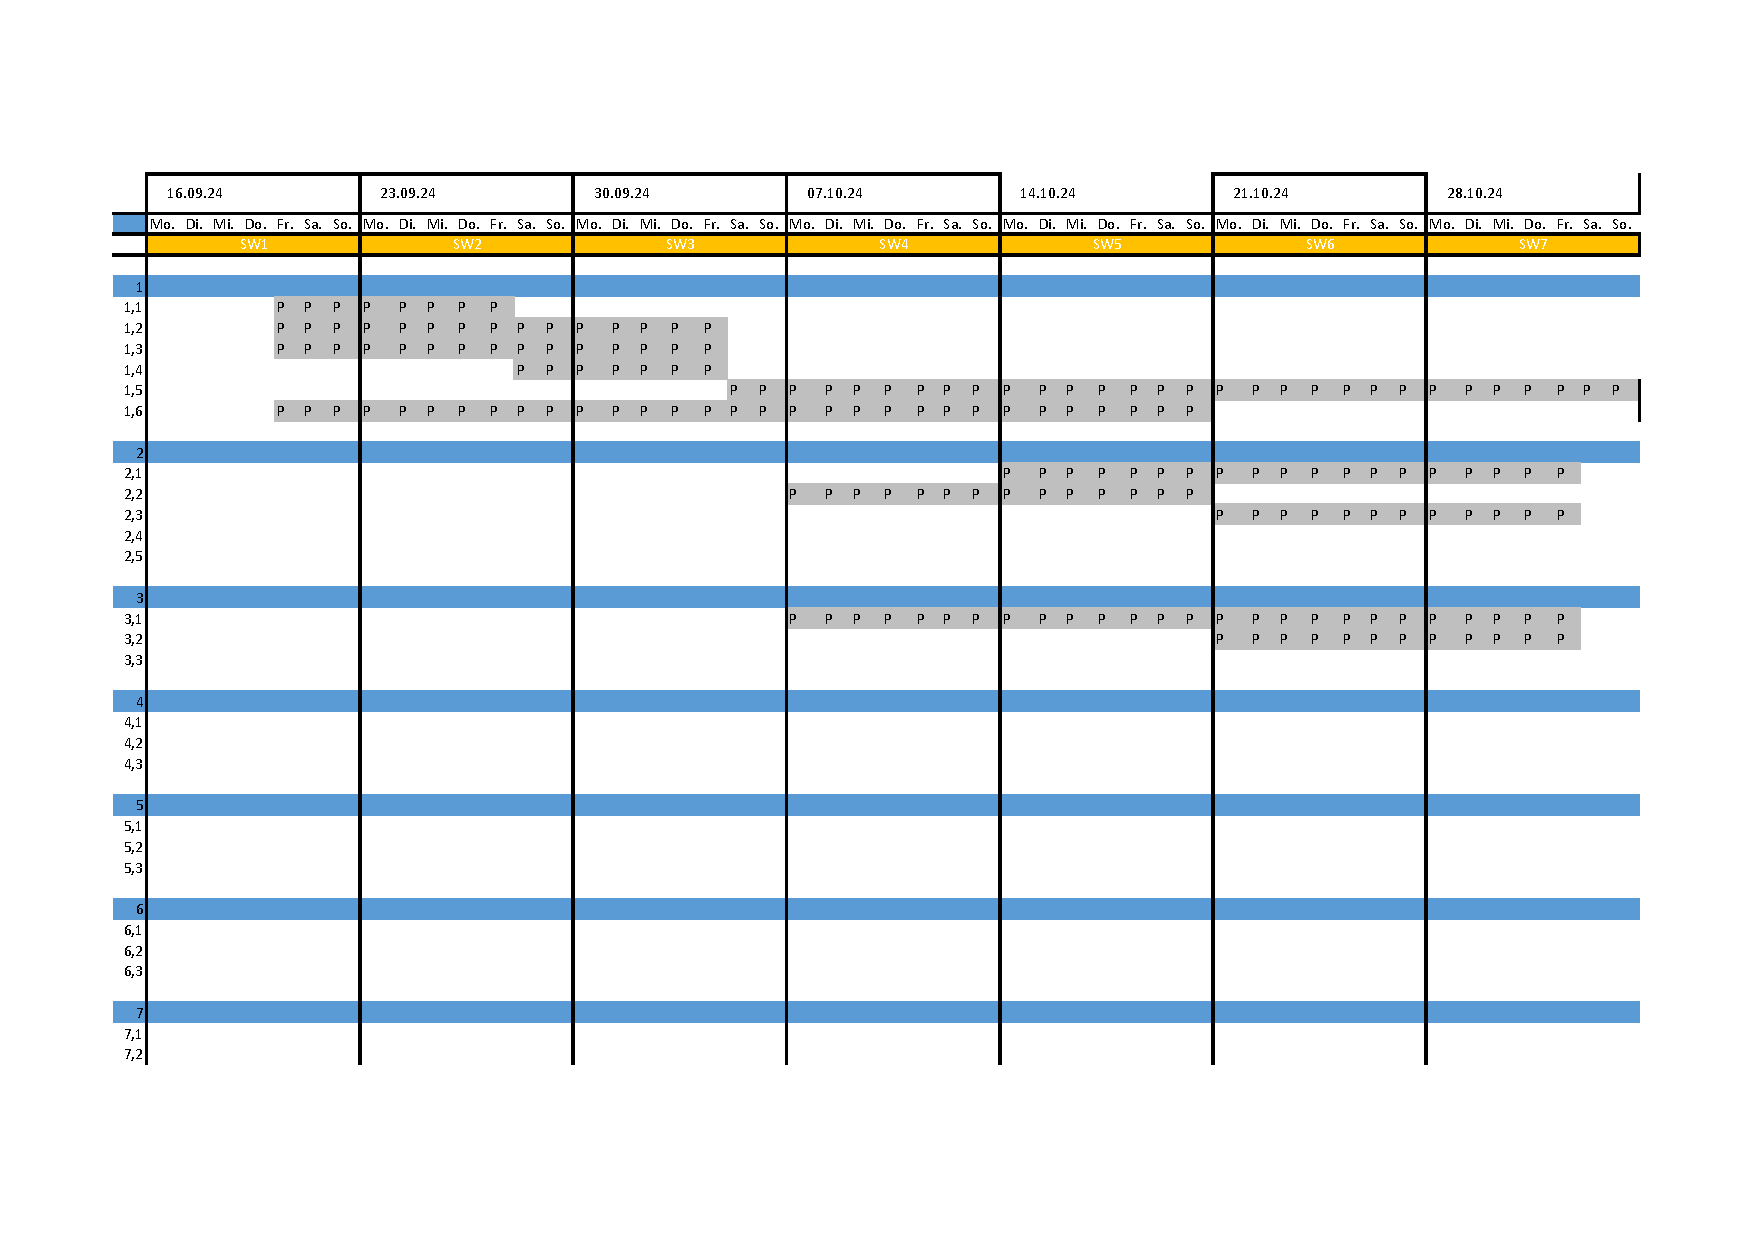
\includepdf[
  landscape=true,
  pages={1-},
  scale=0.9,
  pagecommand={\pagestyle{fancy}}
]{assets/Zeitplan.pdf}

\end{document}